\documentclass{beamer}
\usetheme{Boadilla}
\usecolortheme{dove}

\usepackage[utf8]{inputenc}
\usepackage[T1]{fontenc}
\usepackage{lmodern}

\usepackage[linesnumbered]{algorithm2e}
\DontPrintSemicolon
\setlength{\algomargin}{2em}

\usepackage{tikz}
\usepackage{tikz-3dplot}
\usetikzlibrary{calc, angles, intersections}
\usepackage{pgfplots}

\usepackage{natbib}
\bibliographystyle{alpha}

\usepackage{wrapfig}
\usepackage{multicol}

\title[AMCL6D]{Probabilistic Robot Localization\\in Continuous 3D Maps}
\author{Sebastian Höffner}
\date[2014-12-10]{December 10th, 2014}

\institute[UOS: KBS]
{
  Institute for Computer Science\\
  Knowledge-Based Systems \\ 
  \smallskip
  Institute of Cognitive Science\\
  \bigskip
  University of Osnabrück
}

\begin{document}

\frame{\titlepage}


\section{Localization}

\begin{frame}
  \frametitle{Localization in 6D}
	\begin{center}
    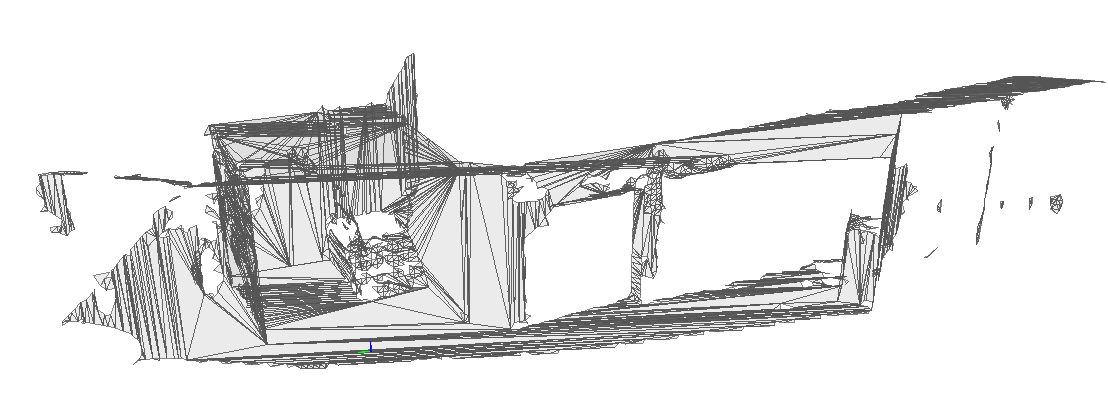
\includegraphics[width=.8\textwidth]{../pics/elvmap}
  \end{center}
\end{frame}

\begin{frame}
  \frametitle{Localization in 1D}
  \begin{figure}
    \centering
    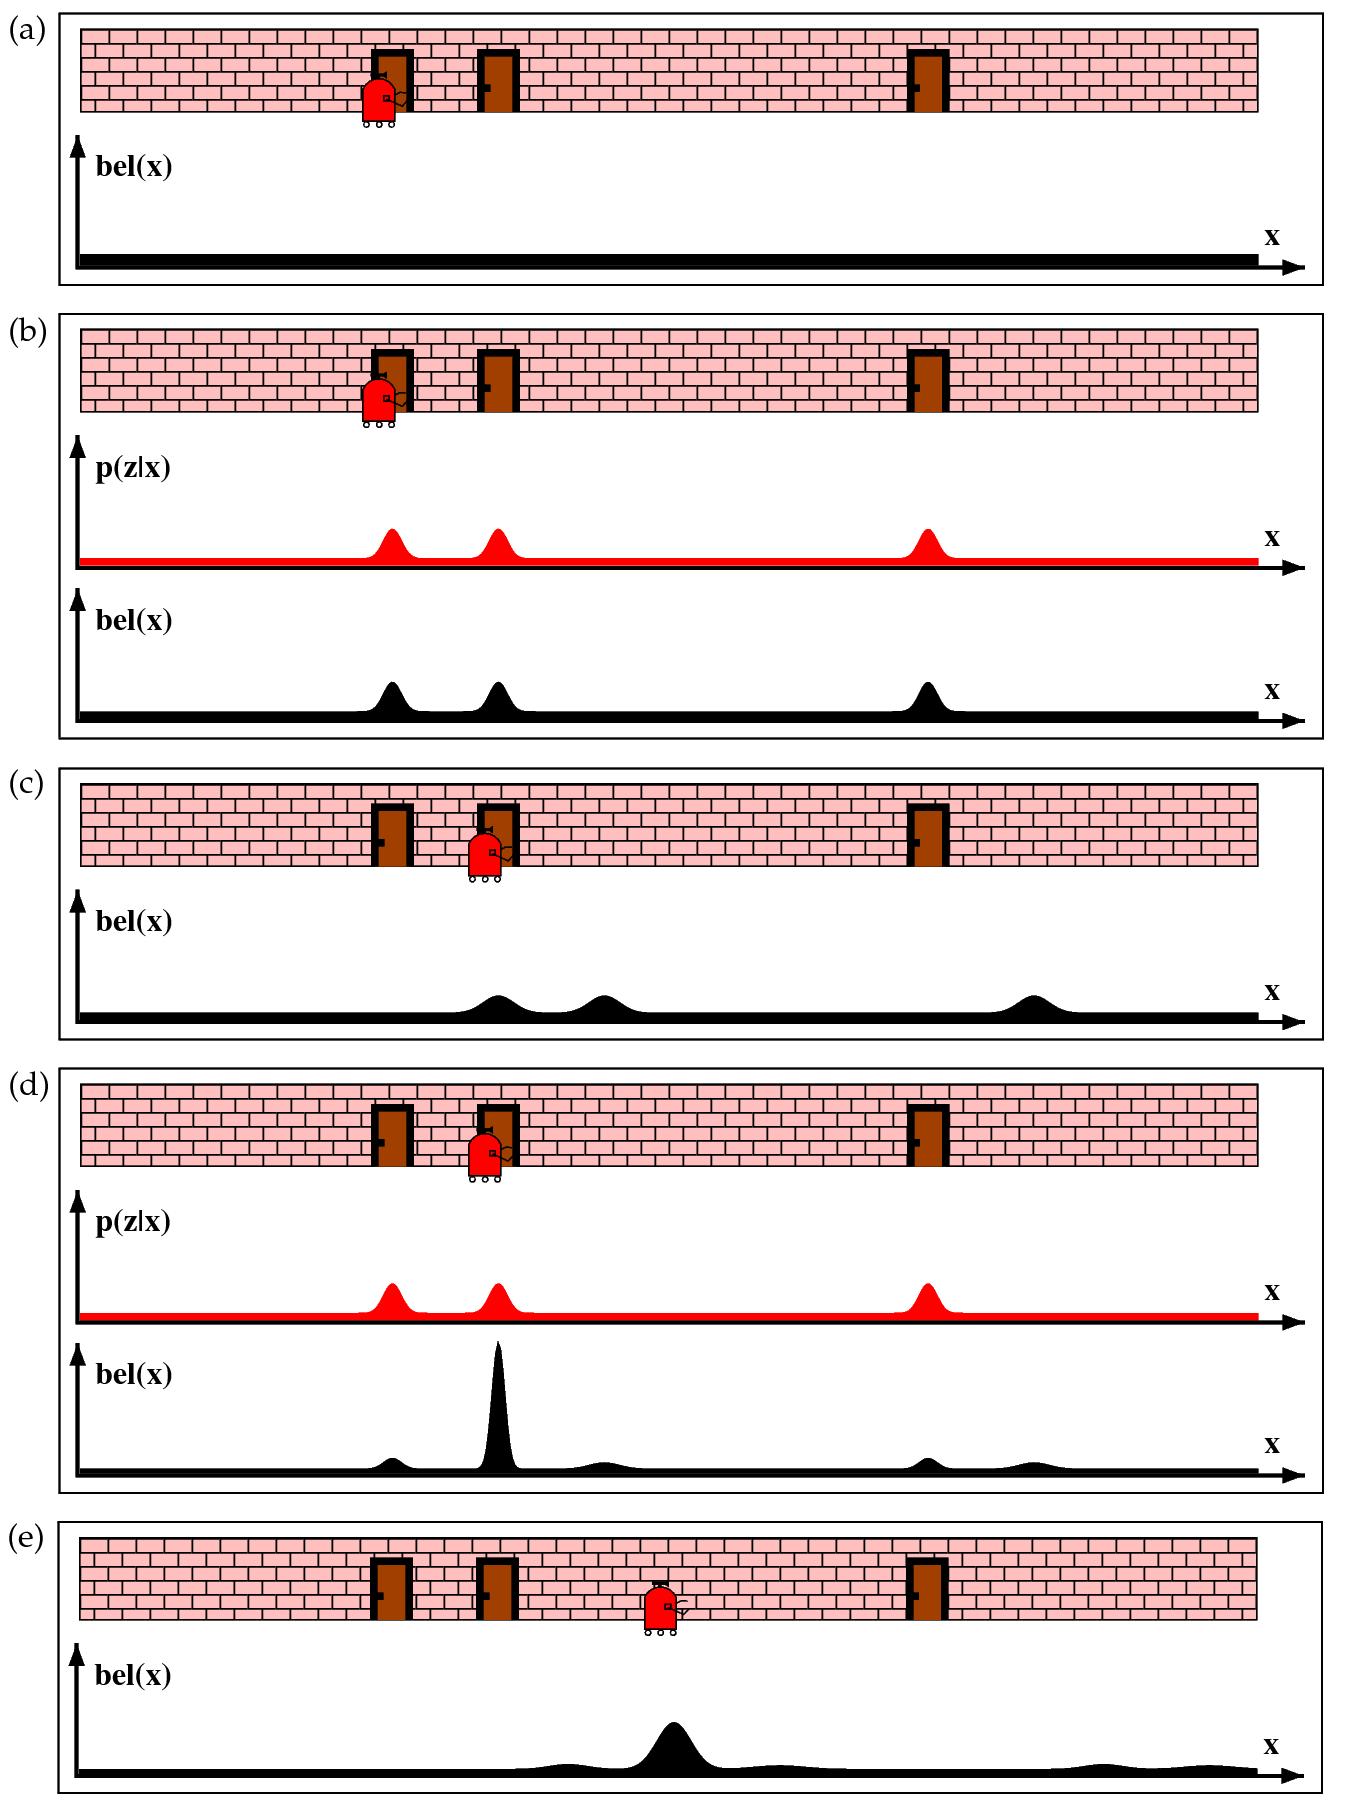
\includegraphics[height=.8\textheight]{../pics/markov_localization}
    \caption{Markov Localization in 1D. From \cite{ThrunBurgardFox:2005}.}
    \label{markovlocalization}
  \end{figure}
\end{frame}


\section{Bayes-/Particlefilter}

\begin{frame}
  \frametitle{Bayes' Theorem}
  \begin{align*}
  P(X|Y) = \frac{P(Y|X)P(X)}{P(Y)}
  \end{align*}
  \begin{align*}
  \text{Posterior} = \frac{\text{Likelihood} \cdot \text{Prior}}{\text{Normalization}}
  \end{align*}
  \begin{itemize}
    \item can be applied iteratively: posterior is the new prior
    \item flat (uninformed) prior/model still leads to real distribution
    \item Markov assumption holds (state N derivable from state N-1)
  \end{itemize}
\end{frame}

\begin{frame}
  \frametitle{Particlefilter}
  \begin{figure}
    \centering
    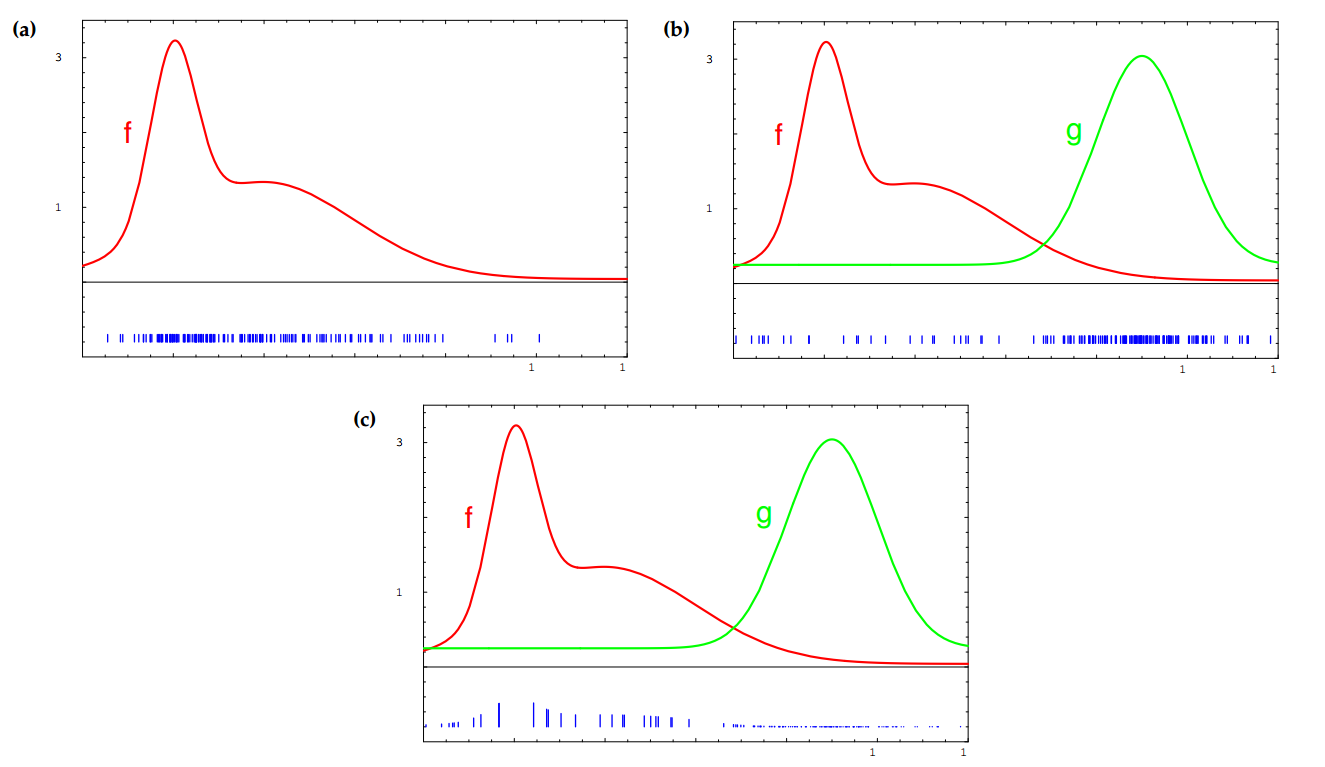
\includegraphics[height=.5\textheight]{../pics/particlefilter}
    \caption{Particles drawn from $g(x)$ are used to approximate $f(x)$. From \cite{ThrunBurgardFox:2005}.}
    \label{particlefilter}
  \end{figure}
	\begin{itemize}
    \item discrete approximation of continuous functions through samples (particles)
    \item reduces complexity while yielding accurate results
    \item particles can be drawn from another function
  \end{itemize}
\end{frame}


\section{AMCL}

\begin{frame}[fragile]
  \frametitle{(A)MCL}
  
  \begin{algorithm}[H]
    \SetKwProg{mcl}{Monte\mathunderscore Carlo\mathunderscore Localization}{}{end}
    \SetKwFunction{appmotion}{apply\mathunderscore motion\mathunderscore model}
    \SetKwFunction{appsensor}{apply\mathunderscore sensor\mathunderscore model}
    \SetKwFunction{replace}{replace\mathunderscore sample}
    \SetKwData{sample}{sample}
    \SetKwData{bel}{belief}
    \mcl{$()$}{
      \ForEach{\sample}{
        \sample.\appmotion{}\;
        \sample.\appsensor{}\;
      }
      \ForEach{\sample}{
        \If{\sample.\bel < $\theta$}{
          \sample.\replace{}\;
        }
      }
    }
    \label{alg:mcl}
    \caption{The basic MCL algorithm.}
  \end{algorithm}
\end{frame}

\begin{frame}[fragile]
  \frametitle{(A)MCL}
  
  \begin{algorithm}[H]
    \SetKwProg{mcl}{Augmented\mathunderscore Monte\mathunderscore Carlo\mathunderscore Localization}{}{end}
    \SetKwFunction{appmotion}{apply\mathunderscore motion\mathunderscore model}
    \SetKwFunction{appsensor}{apply\mathunderscore sensor\mathunderscore model}
    \SetKwFunction{replace}{replace\mathunderscore sample}
    \SetKwData{sample}{sample}
    \SetKwData{bel}{belief}
    \mcl{$()$}{
      \ForEach{\sample}{
        \sample.\appmotion{}\;
        \sample.\appsensor{}\;
      }
      decrease or increase number of samples\;
      \ForEach{\sample}{
        \If{\sample.\bel < $\theta$}{
          \sample.\replace{}\;
        }
      }
    }
    \label{alg:amcl}
    \caption{The AMCL algorithm.}
  \end{algorithm}
\end{frame}

\section{AMCL6D}

\begin{frame}[fragile]
  \frametitle{AMCL6D}
	
  \begin{algorithm}[H]
    \SetKwFunction{mm}{motion\mathunderscore model}
    \SetKwFunction{sm}{sensor\mathunderscore model}
    \SetKwFunction{ev}{evaluation}
    \SetKwFunction{rsrand}{resample\mathunderscore random}
    \SetKwFunction{rsclose}{resample\mathunderscore close}
    \SetKwFunction{sort}{sort}
    \SetKwFunction{rand}{rand}
    \SetKwData{rval}{random}

    \SetKwProg{amcl}{AMCL6D}{}{end}

    \amcl{$(X_{t-1}, u_{t}, m_{t})$} {
      \tcc{Initialize, update motion-/sensor-models:}

      \ForEach{$x \in X_{t}$}{ 
        $x.pose$ = \mm{$x.pose, u_{t}$}\;
        $x.raytrace$ = \sm{$x.pose$}\;
        $x.likelihood$ = \ev{$x.raytrace, m_{t}$}\;
      }

      $\eta = 1 / \sum\limits_{X_{t}}{\left( x.likelihood\ \cdot\ x.probability\right) }$\;

      \ForEach{$x \in X_{t}$}{
        $x.probability = \eta \cdot x.likelihood\ \cdot\ x.probability$\;
      }

      \sort{$X_{t}$}\;
      \ForEach{$x \in X_{t} \wedge x \notin X_{t,best}$}{
        \tcc{Resample}
      }

      \Return{$X_t$}
    }
  \end{algorithm}

\end{frame}


\subsection{Motion Model}

\begin{frame}
  \frametitle{Motion Model}
  
  \begin{multicols}{2}
    \parbox{.5\textwidth}{
      \begin{itemize}
        \item update pose:
        \begin{itemize}
          \item add motion
          \item add noise according to $\Sigma$
        \end{itemize}
      \end{itemize}
      \begin{align*}
        noise &= C^T r + \mu \text{\ \ \ (\cite{Gentle:2005})}\\
        \text{with } C^TC&=\Sigma \text{, $r$: rand(), $\mu = 0$} \\
        q_p &= \text{new QuaternionY(}noise_4\text{)} \\
            &\vdots
      \end{align*}
    }
    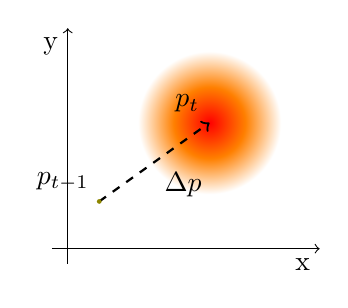
\begin{tikzpicture}[scale=.4]
  % shading
  \pgfdeclareradialshading{ring}{\pgfpoint{0cm}{0cm}}%
  { %
    rgb(  0cm)=(1,0,0);
    rgb( .4cm)=(1,.5,0);
    rgb( .8cm)=(1,1,1);
    rgb(1.0cm)=(1,1,1)%;
  }

  % old and new pos
  \coordinate (oldPos) at(1,1.5);
  \coordinate (newPos) at(4.5,4);
  \coordinate (offset) at(.4,-.5);
  %\coordinate (deltaStart) at($(oldPos)+(offset)$);
  %\coordinate (deltaEnd)   at($(newPos)+(offset)$);

  % uncertainty
  \shade[shading=ring] (newPos) circle (2.5);

  % movement
  \draw[thick,dashed,->] (oldPos) node[above left]  {$p_{t-1}$} 
                              --  node[below right] {$\Delta p$} 
                         (newPos) node[above left]  {$p_{t}$};
  %\draw[thin,|-|] (deltaStart) --  (deltaEnd);

  % certain old pos
  \fill[olive] (oldPos) circle (.075);

  % axes
  \draw[thin, <->] (8,0) node[below left]{x} -| (0, 7) node[below left]{y};
  \draw[thin, -] (-0.5,0) -| (0,-0.5);
\end{tikzpicture}

  \end{multicols}

  \begin{align*}
    (x_t,y_t,z_t)^T &= (x_{t-1},y_{t-1},z_{t-1})^T + \Delta p + (noise_1,noise_2,noise_3)^T&\\
    q_t &= q_{r}q_pq_y\Delta q^{-1}q_{t-1}&
  \end{align*}
  

\end{frame}


\subsection{Sensor Model}

\begin{frame}
  \frametitle{Sensor Model: Raytrace}
	\begin{center}
    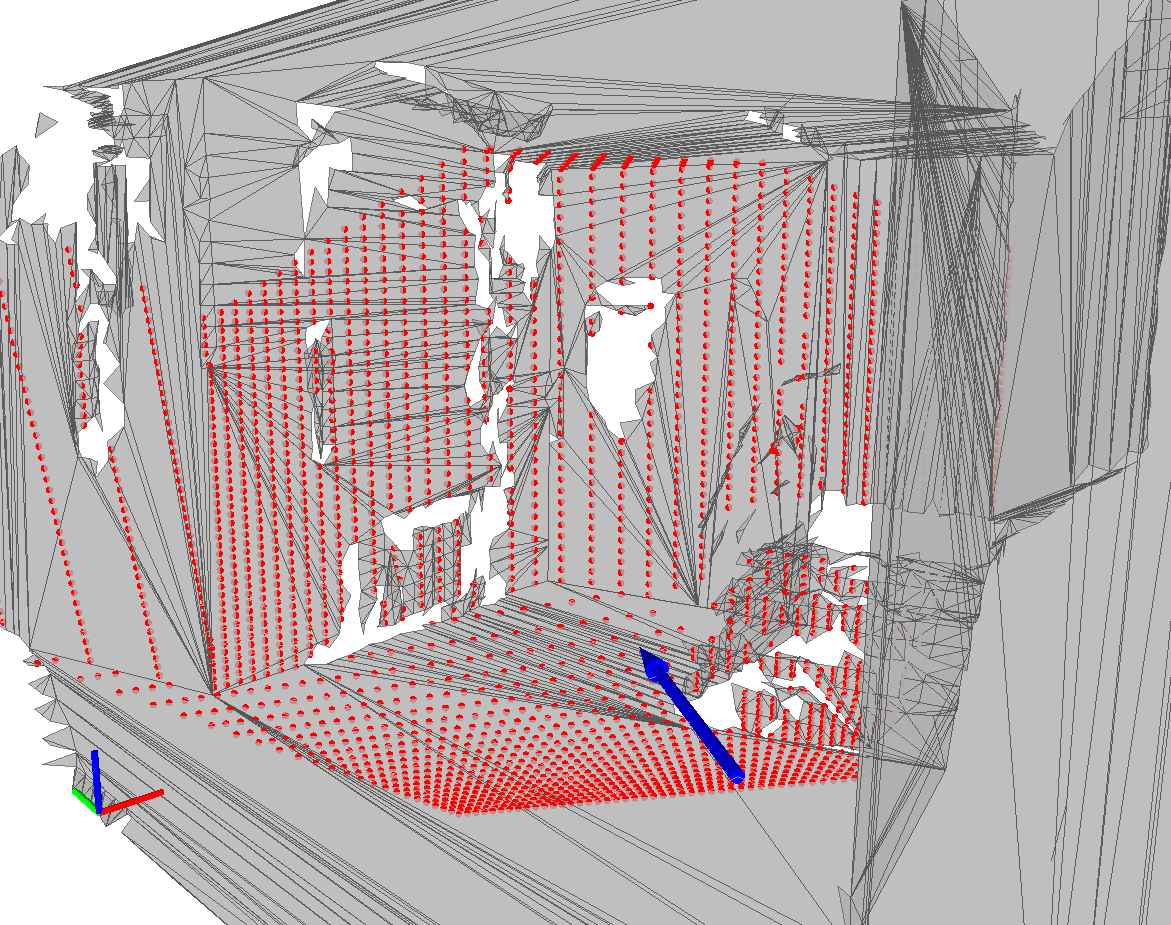
\includegraphics[width=.8\textwidth]{../pics/example_raytrace}
  \end{center}
\end{frame}

\begin{frame}
  \frametitle{Virtual Image Plane}
  \begin{center}
    \begin{figure}[width=.5\textwidth]
      \tdplotsetmaincoords{65}{155}
\begin{tikzpicture}[tdplot_main_coords, scale=.6]

\small
% define plane etc
\def\zMin{-4}
\def\zMax{4}
\def\yMin{-5}
\def\yMax{5}
\def\Focus{-8}

% draw grid
\foreach \y in {\yMin,...,\yMax} \draw[thin, -, gray!20] (\Focus,\y,\zMin) -- (\Focus,\y,\zMax);
\foreach \z in {\zMin,...,\zMax} \draw[thin, -, gray!20] (\Focus,\yMin,\z) -- (\Focus,\yMax,\z);
\draw[->] (\Focus, \yMin-.4,    \zMin) -- (   \Focus, \yMax+.7,    \zMin) node[above right] {y};
\draw[->] (\Focus,    \yMin, \zMin-.4) -- (   \Focus,    \yMin, \zMax+.5) node[below right] {z};
\draw[->] (    .4,    \yMin,    \zMin) -- (\Focus-.5,    \yMin,    \zMin) node[below right] {x} ; 
% draw special ticks
\draw[-] (     0, \yMin, \zMin) -- (     0,    \yMin, \zMin-.2) node[below]       {0};
\draw[-] (\Focus,     0, \zMin) -- (\Focus,        0, \zMin-.2) node[below right] {0};
\draw[-] (\Focus, \yMin,     0) -- (\Focus, \yMin-.2,        0) node[above left]        {0};
\draw[-] (\Focus, \yMin, \zMax) -- (\Focus, \yMin-.2,    \zMax) node[below left]  {\small ($F$, $y_{min}$, $z_{max}$)};
\draw[-] (\Focus, \yMax, \zMin) -- (\Focus,    \yMax, \zMin-.2) node[below left]  {\small ($F$, $y_{max}$, $z_{min}$)};
\node[above left]  at(0, \yMin, \zMin) {\small ($0$, $y_{min}$, $z_{min}$)};

% window (cbr = corner bottom left, t = top, r = right, accordingly)
\coordinate(cbl) at (\Focus, .5*\yMin, .5*\zMin) node[below left]  at (cbl) {$c_{bl}$};
\coordinate(cbr) at (\Focus, .5*\yMax, .5*\zMin) node[below right] at (cbr) {$c_{br}$};
\coordinate(ctr) at (\Focus, .5*\yMax, .5*\zMax) node[above right] at (ctr) {$c_{tr}$};
\coordinate(ctl) at (\Focus, .5*\yMin, .5*\zMax) node[above left]  at (ctl) {$c_{tl}$};

\draw[cyan] (cbl) -- (cbr) -- (ctr) -- (ctl) -- (cbl);

% cam and coordinate in origin
\coordinate(origin) at (0, 0, 0) node[above left] at (origin) {Cam $(0,0,0)$};
\fill[olive] (origin) circle (.1);

% lines and angles (abr = angle bottom right, etc.)
\foreach \c / \a in {cbl/abl,cbr/abr,ctl/atl,ctr/atr}
  \draw[dashed, thin, gray] (origin) -- coordinate[pos=0.4] (\a) (\c);

\draw[thin, -, blue] (atl) to[curve to, relative]                                (abl);
\draw[thin, -, blue] (abl) to[curve to, relative, out=45, in=125, looseness=0.7] (abr);

% this is quite ugly at the moment, but it works
\node[blue] at (-2, 0, .5) {$\phi$};
\node[blue] at (-2.5, 0, -.6) {$\theta$};

% draw help lines for focus/camera
\draw[thin, dashed, gray] (0, \yMin, \zMin) -- (0, 0, \zMin);
\draw[thin, dashed, gray] (origin) -- (0, 0, \zMin) -- (\Focus, 0, \zMin);

% draw distances
\draw[thin, |-|, orange]         (0, 0, \zMin-.3)      -- node[below right] {$F$} (\Focus, 0, \zMin-.3);
\draw[thin, dashed, |-|, orange] ($(ctr) + (0,.4,0)$)  -- node[right]       {$h$} ($(cbr) + (0,.4,0)$);
\draw[thin, dashed, |-|, orange] ($(ctr) + (0,.4,.4)$) -- node[above right] {$w$} ($(ctl) + (0,.4,.4)$);
 
\end{tikzpicture}
    \end{figure}
  \end{center}
\end{frame}

\subsection{Evaluation}

\begin{frame}
	\frametitle{Evaluation: \textsl{k}-NN}
  
  \begin{algorithm}[H]
    \SetKwFunction{kd}{prepare\mathunderscore kd\mathunderscore tree}
    \SetKwFunction{knn}{k\mathunderscore nearest\mathunderscore neighbors}
    \SetKwFunction{ed}{euclidean\mathunderscore distance}
    \SetKwFunction{size}{size}
    \SetKwData{kdtree}{kd\mathunderscore tree}
    \SetKwData{nn}{nearest\mathunderscore neighbor}
    \SetKwData{avgdst}{average\mathunderscore distance}
    \SetKwProg{ev}{evaluation}{}{end}
    \SetKwData{smallval}{$\epsilon$}

    \ev{$(x.raytrace, m_t)$}{
      \kdtree = \kd{$x.raytrace$}\;
      \avgdst = \smallval\;
      \ForEach{$p \in m_t$}{
        \nn = \knn{$p$, \kdtree, 1}\;
        \avgdst += \ed{$p$, \nn} / \size{$m_t$}\;
      }
      \Return{1/\avgdst}
    }
  \end{algorithm}
\end{frame}

\subsection{Particel (Re-)Generation}

\begin{frame}
  \frametitle{Particle (Re-)Generation}
  \begin{itemize}
    \item particle generation
          \begin{itemize}
            \item random positions in 3D paired with
            \item \parbox[t]{.6\textwidth}{random orientation $q=$\\
                  $\left(\sin{2\pi X_1\sqrt{1-X_0}},\cos{ 2\pi X_1 \sqrt{1-X_0}},\right.$\\
                  $\left.\sin{2\pi X_2\sqrt{X_0}},\cos{2\pi X_2\sqrt{X_0}}\right)$\\\cite{gfxgems:1995}}
          \end{itemize}
    \item particle regeneration
          \begin{itemize}
            \item respawn worst (e.g. $40 \%$)
            \item respawn particles with probability $< \Theta$
            \item spawn \textsl{close} or \textsl{random} ($25 \%$ close, $75 \%$ random)
          \end{itemize}
  \end{itemize}
  
\end{frame}

\begin{frame}
  \frametitle{Visualization}
  \begin{center}
    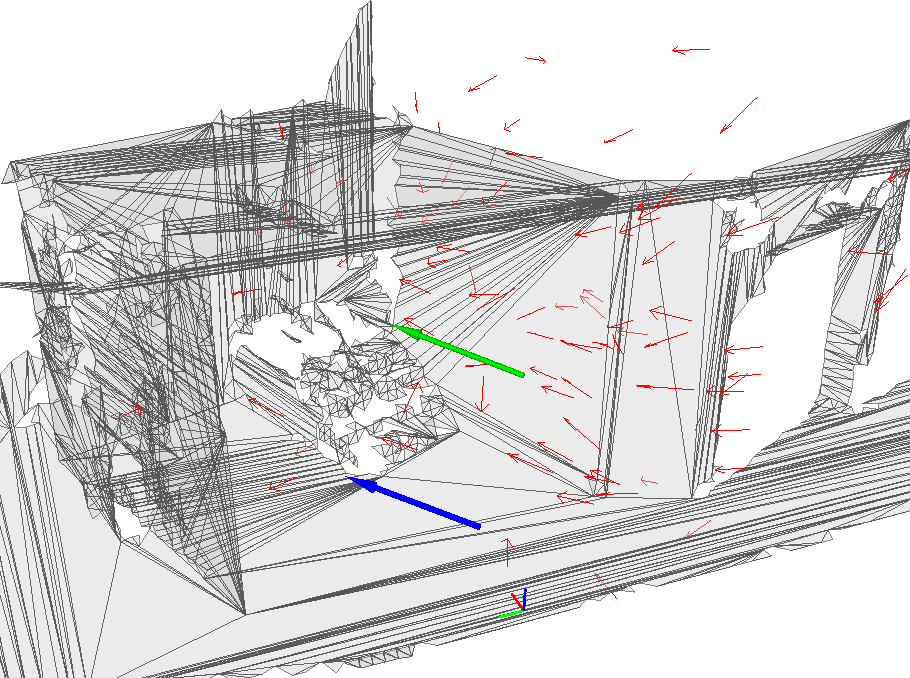
\includegraphics[width=\textwidth]{../pics/amclaction}
  \end{center}
\end{frame}


\section{Results}

\begin{frame}
  \frametitle{Results}
  \begin{figure}%
    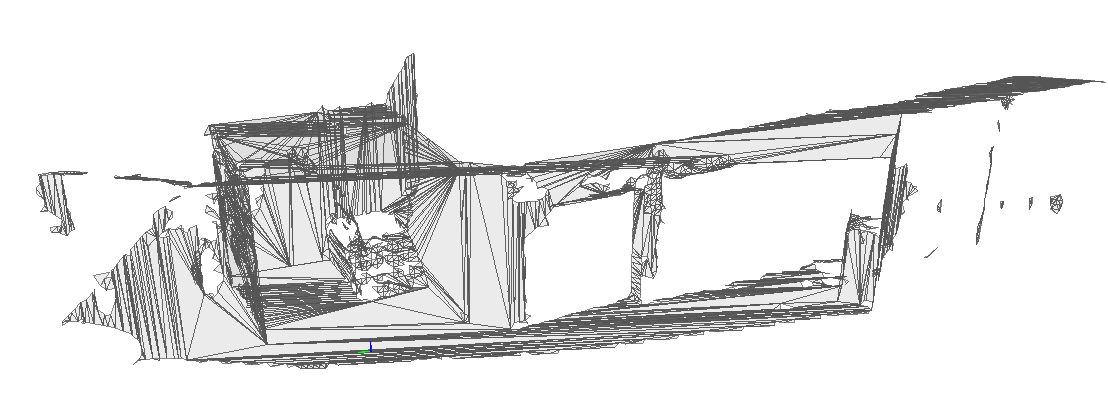
\includegraphics[width=.35\columnwidth]{../pics/elvmap}
    \caption{The elevator doors map}%
    \label{basdlbasld123123kjf97}%
  \end{figure}
  
  \begin{figure}
    \centering
    \begin{tikzpicture}
      \begin{axis}[xlabel={Iterations}, ylabel={Distance},axis lines=left,width=.8\textwidth,height=.45\textwidth]
        \addplot[ultra thin, gray!90] table [x=iter, y=dist, col sep=comma] {../data/elv3.txt};
        \addplot[ultra thin, gray!80] table [x=iter, y=dist, col sep=comma] {../data/elv4.txt};
        \addplot[ultra thin, gray!70] table [x=iter, y=dist, col sep=comma] {../data/elv5.txt};
        \addplot[ultra thin, gray!60] table [x=iter, y=dist, col sep=comma] {../data/elv6.txt};
        \addplot[ultra thin, gray!50] table [x=iter, y=dist, col sep=comma] {../data/elv7.txt};
      \end{axis}
    \end{tikzpicture}
    \caption{Results of the elevator door map.}
    \label{fig:reselv}
  \end{figure}
\end{frame}

\begin{frame}
  \frametitle{Results}
  \begin{figure}%
    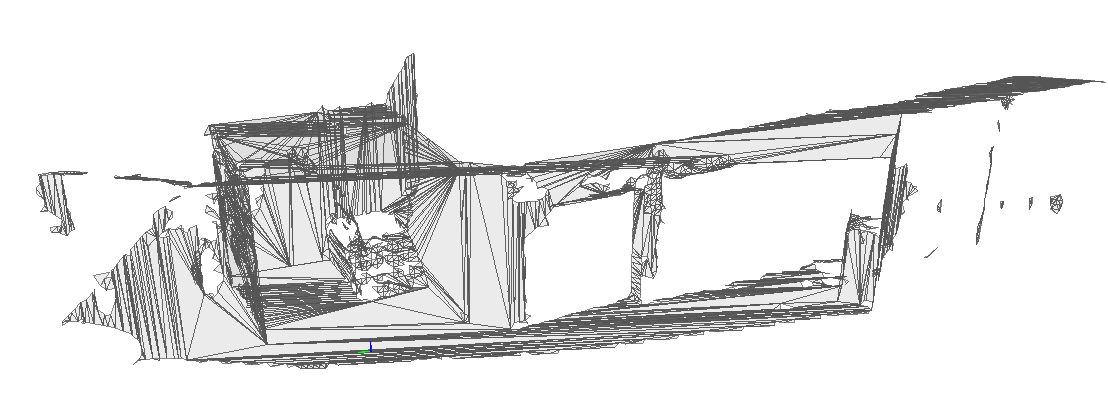
\includegraphics[width=.35\columnwidth]{../pics/elvmap}
    \caption{The elevator doors map}%
    \label{basdlbasld12312397}%
  \end{figure}
  
  \begin{figure}
    \centering
    \begin{tikzpicture}
      \begin{axis}[xlabel={Iterations}, ylabel={Distance},axis lines=left,width=.8\textwidth,height=.45\textwidth,ymax=15]
        \addplot[thin, orange]        table [x=iter, y=avg, col sep=comma]  {../data/elvavg.csv};
      \end{axis}
    \end{tikzpicture}
    \caption{Mean results of the elevator door map.}
    \label{fig:reselztv}
  \end{figure}
\end{frame}

\begin{frame}
  \frametitle{Results}
  \begin{figure}%
    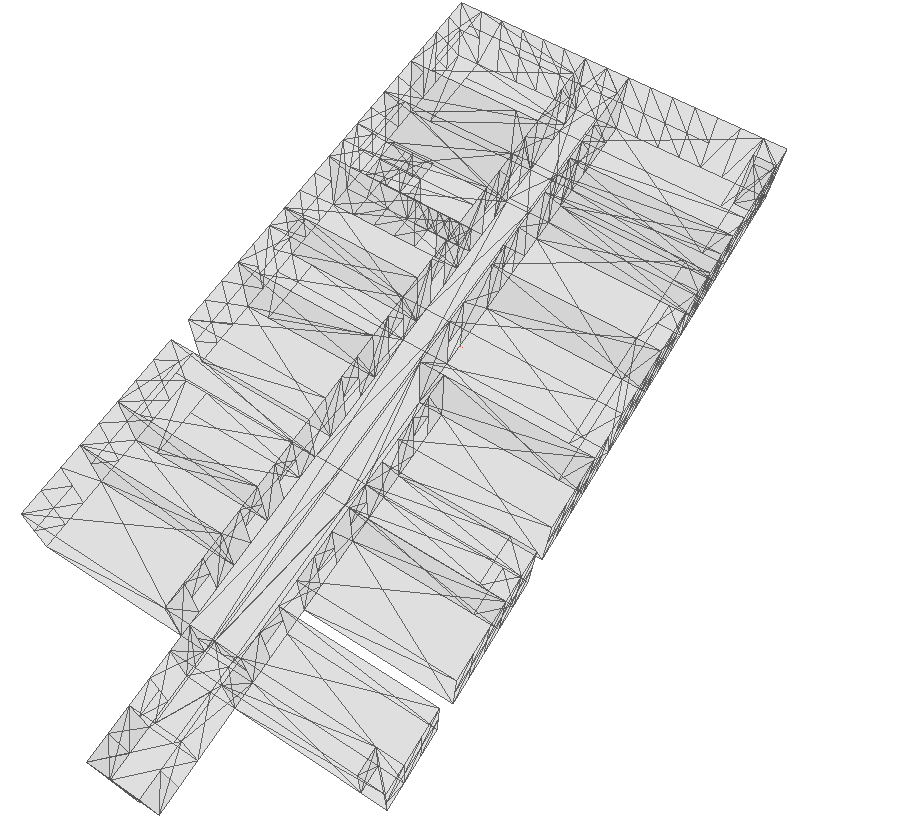
\includegraphics[height=.17\textheight]{../pics/officemap}
    \caption{The office corridor map}%
    \label{basdlbasld123197}%
  \end{figure}
  
  \begin{figure}
    \centering
    \begin{tikzpicture}
      \begin{axis}[xlabel={Iterations}, ylabel={Distance},axis lines=left,width=.8\textwidth,height=.45\textwidth]
        \addplot[ultra thin, gray!90] table [x=iter, y=dist, col sep=comma] {../data/off1.txt};
        \addplot[ultra thin, gray!80] table [x=iter, y=dist, col sep=comma] {../data/off2.txt};
        \addplot[ultra thin, gray!70] table [x=iter, y=dist, col sep=comma] {../data/off3.txt};
        \addplot[ultra thin, gray!60] table [x=iter, y=dist, col sep=comma] {../data/off4.txt};
        \addplot[ultra thin, gray!50] table [x=iter, y=dist, col sep=comma] {../data/off5.txt};
      \end{axis}
    \end{tikzpicture}
    \caption{Results of the office corridor map.}
    \label{fig:reshgelv}
  \end{figure}
\end{frame}

\begin{frame}
  \frametitle{Results}
  \begin{figure}%
    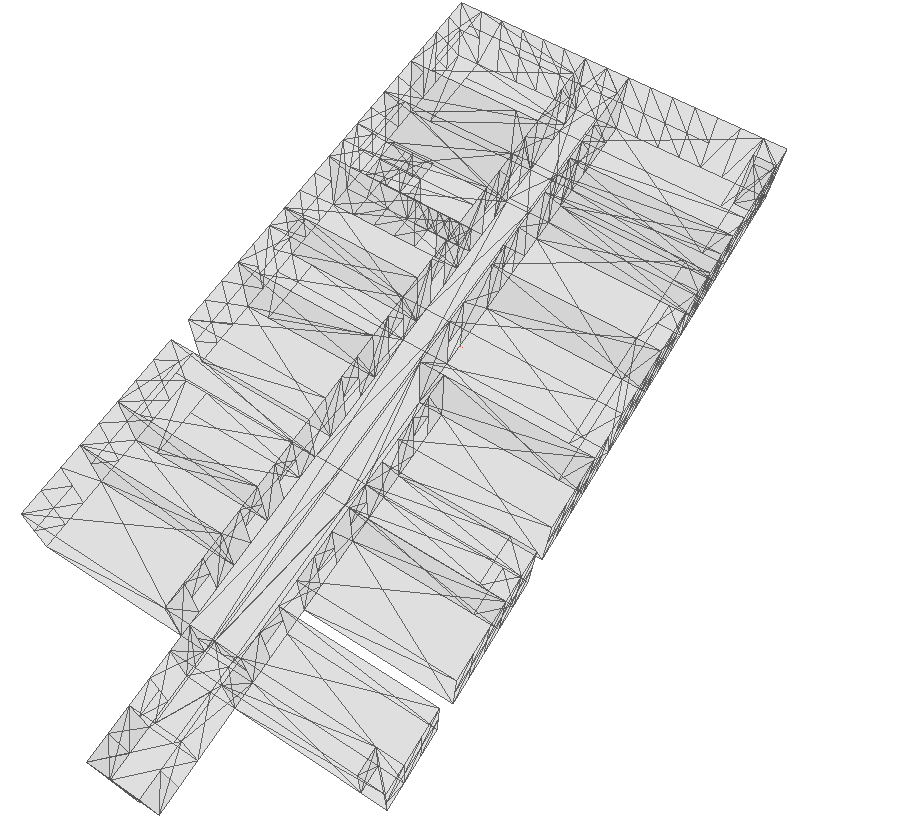
\includegraphics[height=.17\textheight]{../pics/officemap}
    \caption{The office corridor map}%
    \label{baskjf97}%
  \end{figure}
  
  \begin{figure}
    \centering
    \begin{tikzpicture}
      \begin{axis}[xlabel={Iterations}, ylabel={Distance},axis lines=left,width=.8\textwidth,height=.45\textwidth,ymax=20]
        \addplot[thin, orange]        table [x=iter, y=avg, col sep=comma]  {../data/offavg.csv};
      \end{axis}
    \end{tikzpicture}
    \caption{Mean results of the office corridor map.}
    \label{fig:res4567elv}
  \end{figure}
\end{frame}

\begin{frame}
  \frametitle{Results}

  \begin{figure}
    \centering
    \begin{tikzpicture}
      \begin{axis}[xlabel={Iterations}, ylabel={Distance},axis lines=left,width=.8\textwidth,height=.4\textwidth, legend style={at={(.5,1)},anchor=north}]
        \addplot[red]    table [x=iter, y=avg, col sep=comma] {../data/elvsavg.csv};
          \addlegendentry{30x20}
        \addplot[blue] table [x=iter, y=avg, col sep=comma] {../data/elvavg.csv};
          \addlegendentry{65x45}
        \addplot[olive]  table [x=iter, y=avg, col sep=comma] {../data/elvhavg.csv};
          \addlegendentry{100x80}
      \end{axis}
    \end{tikzpicture}
    \caption{Impact of Resolutions}
    \label{baskjf97asdasfgafsd}%
  \end{figure}
\end{frame}

\begin{frame}
  \frametitle{Results}
  \framesubtitle{Raytracer Performance}
  \begin{figure}
    \centering
    \begin{tikzpicture}
      \begin{axis}[ymin=0,ymax=1,enlargelimits=0,xlabel={Different trials},ylabel={Ray tracing time / total time}, ybar interval = 0.4]
        \addplot[green!20!black,fill=green!50!white] table[x=trial,y=per,col sep=comma] {../data/rtres_100.csv}; 
      \end{axis}
      \begin{axis}[ymin=0,ymax=1,enlargelimits=0,axis lines=none, ybar interval = 0.4]
          \addplot[red!20!black,fill=red!50!white] table[x=trial,y=per,col sep=comma] {../data/rtres.csv};
      \end{axis}
    \end{tikzpicture}
    \caption{Comparison of total time to ray trace time.}
    \label{fig:rttimebenchmark}
  \end{figure}
\end{frame}

\begin{frame}
	\frametitle{Future}
  
  \begin{itemize}
    \item Dynamic/Adaptive respawn
    \item Raytracer computation times
    \item Evaluation functions
  \end{itemize}
\end{frame}


\begin{frame}
	\frametitle{Questions?}
\end{frame}


\section{Bibliography}

\begin{frame}
  \frametitle{Bibliography}
  \bibliography{thesis_bibliography}
\end{frame}


\end{document}